\chapter{Polyphonic Mode}

\section{Voice Select Page}
The voice select page is used to assign MD tracks as polyphonic voices.\\\\
The TI is used to select voices\\\\
\fbox{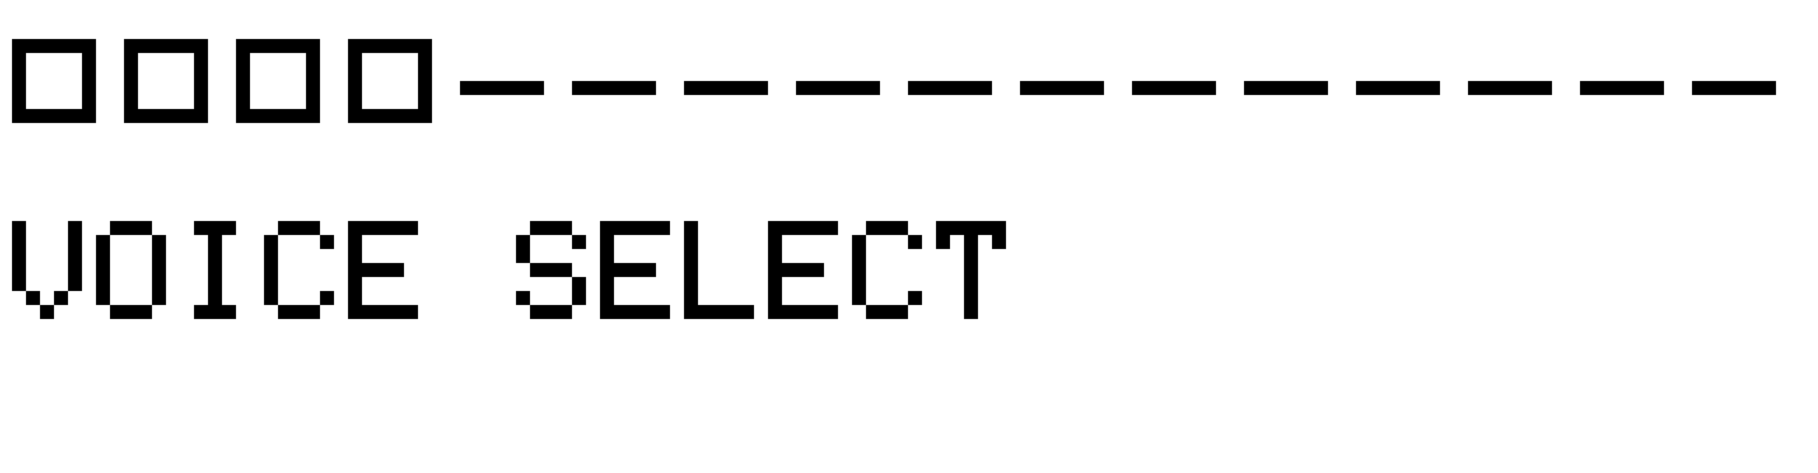
\includegraphics[scale=.40]{voice_select_page.png}}\\\\
\textit{To open the voice select page:\\\\
Enter \textbf{GlobalSettings-->MD-->POLY CONFIG}. Or press \textbf{[Save]} + \textbf{[Write]} from  Chromatic Page}
\section{Voice modes}

When in the Chromatic Page, the Machinedrum's current active track will be used as a monophonic voice.\\
\\
If the current active track is part of the Polyphonic track selection \textbf{POLY} mode will be activated; the MD will be played polyphonically using voices selected from the \textbf{POLY Page.}\\
\\
When POLY mode is active, tracks become 'linked'. Track length and parameter changes will be synchronised across the voices. In addition pressing \textbf{Write} from thePTC Page will clear all recorded sequencer data from the poly tracks.
\section{Setting up Poly Mode}
For best results, make sure that the tracks designated as a poly voice are all set to the same machine type on the MD. You can quickly copy one track to another using the MD's\textbf{Func} + \textbf{Copy/Paste} buttons.\\\\
In order for the Megacommand to synchronise with the MD's current kit/track settings, re-enter the MCL page by tapping \textbf{PageSelect} each time you change a machine type on the MD.
\newpage
\section{Machinedrum External MIDI}
The MD can be played chromatically using an attached MIDI keyboard/sequencer connected to MIDI input port 2.
To enable/disable control from an external device you must change the Megacommand's \textbf{Global Settings->Machinedrum->CTRL CHAN} setting from INT (internal) to a desired MIDI channel or OMNI (all channels).\\
\\
When external control mode is enabled, the trigger interface will be disabled.\\
\\
You can control the voice parameters using MIDI CC messages. CC 16 to 39 control MD parameters 1 to 24 on the active track, or across all polyphonic tracks.

